\subsection{Simulación del proceso evolutivo}
La simulación del proceso evolutivo del mosquito del Aedes aegypti, presentado previamente en la
\secref{sec:cap4-simulador-proceso-evolutivo}, es el encargado de simular los efectos temperatura
en el ciclo de vida del mosquito.

La población inicial es obtenida mediante la cantidad de larvas observadas en los puntos de
control que corresponden a la muestra utilizada para el estudio. Por cada larva observada,
en un punto de control ubicado en las coordenadas geográficas, $(x, y)$, se inicializa un individuo
con las mismas coordenadas del punto de control de origen.

\begin{figure}[!htpb]
\centering
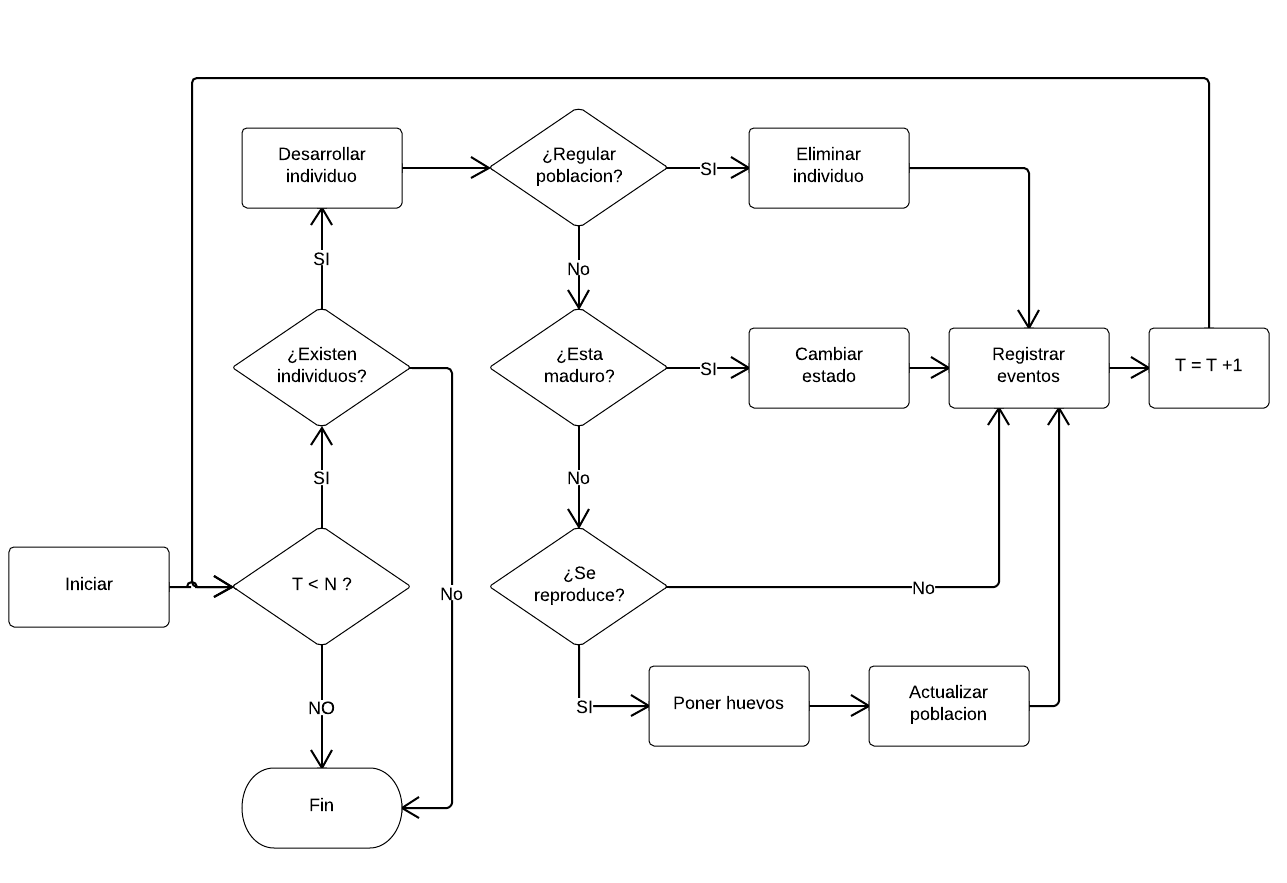
\includegraphics[width=1\textwidth]{capitulo-5/graphics/algoritmo-evolutivo.png}
\caption{\label{fig:cap-5-alg-evolutivo} Algoritmo del simulador del proceso evolutivo.}
\end{figure}

En la \figref{fig:cap-5-alg-evolutivo}, se presenta el algoritmo del simulador del proceso
evolutivo, que es considerado como un proceso iterativo. El simulador inicia tomando como
parámetros de entrada la población inicial, y el periodo de simulación, representado por $T$. El
proceso se ejecutará siempre y cuando se cumplan las siguientes condiciones : el periodo de
simulación, $T$, no haya finalizado y que la población cuente con individuos para su procesamiento.
En el caso de que no se cumplan algunas de las condiciones mencionadas anteriormente, el proceso
de simulación finalizará.

El desarrollo de los individuos se encarga de calcular las tasas de desarrollo correspondientes
para cada etapa de su ciclo de vida (Ver \secref{subsec:cap4-tasas de desarrollo}
), con el fin de estimar su desarrollo considerando las condiciones climáticas. El cambio de
estado es consecuencia de la finalización de la etapa de desarrollo del individuo, donde el
individuo ya está listo para pasar a la siguiente etapa de su ciclo de desarrollo.


La regulación de la población es la encargada de calcular las tasas de mortalidad diaria,
correspondientes a cada etapa del ciclo de desarrollo del individuo (Ver
\secref{subsec:cap4-mortalidad}), con el fin de reducir el tamaño de la población debido a la
mortalidad diaria de los individuos.

Si el individuo en cuestión corresponde a una hembra adulta inseminada, entonces esta se encuentra
en fase reproductiva. La postura de huevos se realiza respetando la tasa de desarrollo del ciclo
gonotrófico de las hembras (Ver \secref{subsec:cap4-ciclo-gontrofico-ovipostura}). Si la hembra
adulta ovipone, los huevos son añadidos a la población como individuos en un estado inicial de
\textit{HUEVO}.

Las efectos de la temperatura, en cada individuo son registrados mediante un proceso que se
encarga de almacenar, en una base de datos, la información correspondiente, de cada individuo para
su posterior análisis. Estos efectos pueden desencadenar en una serie de eventos en el individuo
como : eclosión de huevos, mortalidad de larvas, emergencia de pupas, muerte de pupas, emergencia
de adultos, muerte de adultos, ovipostura y dispersión de los adultos.
